\documentclass{article}
\usepackage{tikz}
\usepackage{amssymb}
\usepackage{amsthm}
\usepackage{amsmath}
\usepackage{mathabx}
\usepackage{listings}
\usepackage{bbm}
\usepackage{caption}
\usepackage{natbib}
\usepackage{float}
\usepackage{hyperref}
\usepackage{setspace}
\usepackage[margin = 1 in]{geometry}
\usepackage{tcolorbox}
\usetikzlibrary{patterns,automata,positioning,arrows}
\title{Strategy Free Machine Learning}
\author{-}
\date{\today}
\hbadness=99999

\begin{document}
\newtheorem{thm}{Theorem}
\newtheorem{cor}{Corollary}
\newtheorem{lem}{Lemma}
\newtheorem{prop}{Proposition}
\newtheorem{conj}{Conjecture}
\newtheorem{algo}{Algorithm}
\newtheorem{obs}{Observation}
\newtheorem{clm}{Claim}
\theoremstyle{definition}
\newtheorem{df}{Definition}
\newtheorem{eg}{Example}
\newtheorem{asm}{Assumption}
\newtheorem{cond}{Condition}
\theoremstyle{remark}
\newtheorem{rmk}{Remark}
\maketitle \onehalfspacing \allowdisplaybreaks \raggedbottom


\section{Literature Review} 
Previous work on mechanism design for machine learning with strategic data sources focus on designing robust algorithms to incentivize the data providers to report their private data truthfully. Their models mainly differ in the objective and the possible actions of the data providers (agents) and the machine learner (principal).
\begin{itemize}
\item The first group of papers focuses on principal-agent problems in which each agent's private data point is the agent's type that the agent cannot change. The only action the agents can take is whether to report their private information truthfully.
\end{itemize}
\begin{enumerate}
\item Some models assume the agents' feature vectors are public, but their labels are private. \citet*{perote2004strategy}, \citet*{chen2018strategyproof}, and \citet*{gast2013linear} focus on strategy-proof linear regression algorithms and introduced clockwise repeated median estimators, generalized resistant hyperplane estimators, and modified generalized linear squares estimators. \citet*{dekel2010incentive} investigates the general regression problem with empirical risk minimization and absolute value loss. All the previously mentioned papers assume the labels are continuous variables (regression problems), and \citet*{meir2012algorithms} assumes the labels are discrete variables (classification problems) and proposes a class of random dictator mechanisms.
\item Some models assume the agents' feature vectors are also private. \citet*{chen2019grinding} investigates such problems for linear regressions.
\item Other models do not distinguish between feature vectors and labels. Each agent has a private valuation. These problems are usually modeled as facility locations problems and the solution involves some variant of the Vickrey-Clarke-Groves or Meyerson auction. These include \citet*{dutting2017optimal}, \citet*{golowich2018deep}, \citet*{epasto2018incentive}, and \citet*{procaccia2009approximate}.
\end{enumerate}

\begin{itemize}
\item The second group papers focus on moral-hazard problems in which each agent does not have a type but they can choose an action (with a cost) that affects the probability of obtaining the correct label. \citet*{richardsonprivately} focuses on the linear regression problem in this scenario, and \citet*{cai2015optimum} and \citet*{shah2016double} investigates the problem for more general machine learning problems. \citet*{mihailescu2010strategy} also discusses a similar problem for general machine learning algorithms.
\item The last group of papers uses machine learning or robust statistics techniques without game-theoretic models. This group of papers include \citet*{dekel2009vox}, \citet*{dekel2009good}.
\end{itemize}



\section{Model} 

\subsection{Maximum Likelihood Estimation}
There are $n $ strategic agents each providing the label of one data point to the principal. The principal is the learner and builds a machine learning model based on the data points provided by the agents, in particular, we assume the principal is training a softmax regression for multi-class classification. An agent, $i $, has publicly known feature vector, $x^{\left(i\right)}$, and a private discrete label, $y^{\left(i\right)}$. The objective of the agent is to maximize the probability that her data point is labeled correctly by the principal's model, and the agent can choose to report $\hat{y} ^{\left(i\right)}$ to achieve the objective, with possibly $\hat{y} ^{\left(i\right)} \neq  y^{\left(i\right)}$. The objective of the principal is to minimize the loss from the data set with the correct labels.
\newline \newline


\subsection{Partial Loss Function Derivations}
A dataset is incentive incompatible if,
\begin{align*}
\mathbb{P}\left\{Y = y^{\left(i\right)} | w^\star , x^{\left(i\right)}\right\} &\leq  \mathbb{P}\left\{Y = y^{\left(i\right)} | \hat{w}, x^{\left(i\right)}\right\},
\end{align*}
where,
\begin{align*}
w^\star  &= \arg\displaystyle\max_{w} \log\left(\mathbb{P}\left\{Y = y^{\left(i\right)} | w, x^{\left(i\right)}\right\}\right) + C_{-i}\left(w\right),
\\ \hat{w} &= \arg\displaystyle\max_{w} \log\left(\mathbb{P}\left\{Y = \hat{y} | w, x^{\left(i\right)}\right\}\right) + C_{-i}\left(w\right).
\end{align*}
The function $C\left(w\right) $ summarizes the loss due to other agents, assuming they are reporting labels truthfully,
\begin{align*}
C_{-i}\left(w\right) &= \displaystyle\sum_{i' \neq  i} \log\left(\mathbb{P}\left\{Y = y^{\left(i'\right)} | w, x^{\left(i'\right)}\right\}\right).
\end{align*}
Suppose the function $L $ is globally convex, differentiable, etc, then the problem translates to the first derivative condition,
\begin{align*}
\dfrac{\nabla _{w} \mathbb{P}\left\{Y = y^{\left(i\right)} | w^\star , x^{\left(i\right)}\right\}}{\mathbb{P}\left\{Y = y^{\left(i\right)} | w^\star , x^{\left(i\right)}\right\}} + \nabla _{w} \left(C_{-i}\left(w^\star \right)\right) &= 0,
\\ \dfrac{\nabla _{w} \mathbb{P}\left\{Y = \hat{y} | \hat{w}, x^{\left(i\right)}\right\}}{\mathbb{P}\left\{Y = \hat{y} | \hat{w}, x^{\left(i\right)}\right\}} + \nabla _{w} \left(C_{-i}\left(\hat{w}\right)\right) &= 0.
\end{align*}
For logistic regression with weights $w_{c}, c = 1, 2, ..., K, $
\begin{align*}
\mathbb{P}\left\{Y = c | w, x\right\} &= \dfrac{e^{w_{c}^{T} x + b_{c}}}{\displaystyle\sum_{c'} e^{w_{c'}^{T} x + b_{c'}}},
\\ \nabla _{w_{c}} \mathbb{P}\left\{Y = c | w, x\right\} &= \dfrac{e^{w_{c}^{T} x + b_{c}} \displaystyle\sum_{c' \neq  c} e^{w_{c}^{T} x + b_{c}}}{\left(\displaystyle\sum_{c'} e^{w_{c'}^{T} x + b_{c'}}\right)^{2}} x.
\\ \nabla _{w_{c}} \mathbb{P}\left\{Y = \hat{c} \neq  c | w, x\right\} &= \dfrac{e^{w_{c}^{T} x + b_{c}} e^{w_{\hat{c}}^{T} x + b_{\hat{c}}}}{\left(\displaystyle\sum_{c'} e^{w_{c'}^{T} x + b_{c'}}\right)^{2}} x.
\end{align*}
The derivative conditions implies,
\begin{align*}
\left(1 - \mathbb{P}\left\{Y = c | w^\star , x^{\left(i\right)}\right\}\right) x^{\left(i\right)} + \nabla _{w_{c}} \left(C_{-i}\left(w^\star \right)\right) &= 0, c = y^{\left(i\right)},
\\ \left(\mathbb{P}\left\{Y = c | w^\star , x^{\left(i\right)}\right\}\right) x^{\left(i\right)} + \nabla _{w_{c}} \left(C_{-i}\left(w^\star \right)\right) &= 0, c \neq  y^{\left(i\right)},
\end{align*}
same for the expression with $\hat{w}$.
\\* Substitute into the incentive incompatibility condition,
\begin{align*}
\nabla _{w_{y^{\left(i\right)}j}} \left(C_{-i}\left(w^\star \right)\right)) x^{\left(i\right)}_{j} &\leq  \nabla _{w_{y^{\left(i\right)}j}} \left(C_{-i}\left(\hat{w}\right)\right) x^{\left(i\right)}_{j}, j = 1, 2, ..., m. 
\end{align*}


\subsection{Continuous Y Derivations}
\begin{tcolorbox}[colback = white]
Envolope theorem version of the derivation.
\end{tcolorbox}
Specifically, for the softmax regression, the objective of agent $i $ with $x^{\left(i\right)} \in \mathbb{R}^{m}$ and $y^{\left(i\right)} \in \left\{1, 2, ..., k \right\}$ is,
\begin{align*}
&  \displaystyle\max_{\hat{y} \in \left\{1, 2, ..., k \right\}} \mathbb{P}\left\{Y = y^{\left(i\right)} | w, x^{\left(i\right)}\right\},
\end{align*}
where,
\begin{align*}
&  \mathbb{P}\left\{Y = c | w, x^{\left(i\right)}\right\} = \dfrac{e^{z_{c}^{\left(i\right)}}}{\displaystyle\sum_{c'=1}^{k} e^{z_{c'}^{\left(i\right)}}},
\\ &  z_{c}^{\left(i\right)} = \displaystyle\sum_{j=1}^{m} w_{j,c} x_{j}^{\left(i\right)} + b_{c} , \text{\;for\;} c \in \left\{1, 2, ..., k\right\}.
\end{align*}
The learner maximizes the likelihood of the data.
\begin{align*}
&\displaystyle\max_{w} \displaystyle\sum_{i=1}^{n} \log\left(\mathbb{P}\left\{Y = \hat{y} ^{\left(i\right)} | w, x^{\left(i\right)}\right\}\right),
\end{align*}
where $w $ is the $m  \times \left(k  + 1\right)$ weight matrix that includes the bias terms for the softmax regression.
\newline \newline
This formulation does not permit $\hat{y} ^{\left(i\right)}$ to be a continous variable, but if we rewrite the optimization problem as the maximization of the cross entropy, then we could treat $\hat{y} ^{\left(i\right)}$ as a continous multinomial distribution,
\begin{align*}
&\displaystyle\min_{w} \displaystyle\sum_{i=1}^{n} \displaystyle\sum_{c=1}^{k} \hat{-y}_{c}^{\left(i\right)} \log\left(\mathbb{P}\left\{Y = c | w, x^{\left(i\right)}\right\}\right)
\end{align*}
Use envolope theorem and assume $w^\star \left(\hat{y} ^{\left(i\right)}\right)$ is the optimal weights. The objective function is,
\begin{align*}
\mathcal{L}\left(w, \hat{y} ^{\left(i\right)}\right) &= \displaystyle\sum_{i=1}^{n} \displaystyle\sum_{c=1}^{k} \hat{-y}_{c}^{\left(i\right)} \log\left(\mathbb{P}\left\{Y = c | w, x^{\left(i\right)}\right\}\right),
\end{align*}
and the value function is,
\begin{align*}
\mathcal{L}^\star \left(\hat{y} ^{\left(i\right)}\right) &= \displaystyle\sum_{i=1}^{n} \displaystyle\sum_{c=1}^{k} \hat{-y}_{c}^{\left(i\right)} \log\left(\mathbb{P}\left\{Y = c | w^\star , x^{\left(i\right)}\right\}\right),
\end{align*}
apply envolope theorem,
\begin{align*}
\dfrac{\partial \mathcal{L}^\star \left(\hat{y} ^{\left(i\right)}\right)}{\partial \hat{y} ^{\left(i\right)}} &= -\log\left(\mathbb{P}\left\{Y = \hat{y} ^{\left(i\right)} | w^\star , x^{\left(i\right)}\right\}\right)
\\ &> 0.
\end{align*}
\begin{tcolorbox}[colback = white]
Gradient descent version of the derivation.
\end{tcolorbox}
One iteration of the gradient descent with learning rate $\eta$ is given by,
\begin{align*}
w'_{j,c} &= w_{j,c} - \eta x_{j}^{\left(i\right)} \left(\mathbb{P}\left\{Y = c | x^{\left(i\right)}\right\} - \mathbbm{1}_{\hat{y} = c}\right).
\end{align*}
We start by treating $y^{\left(i\right)}$ as a continuous distribution over $\left\{1, 2, ..., k \right\}$ and investigate if reporting $\hat{y} \neq  y^{\left(i\right)}$ increases the probability that the model classifies $x^{\left(i\right)}$ as $y^{\left(i\right)}$. Denote the probability $\mathbb{P}\left\{Y^{\left(i\right)} = c\right\}$ by $y_{c}^{\left(i\right)}$ (slight abuse of notation). Then $\begin{bmatrix} y_{1}^{\left(i\right)} & y_{2}^{\left(i\right)} & ... & y_{k}^{\left(i\right)} \end{bmatrix} ^{T} \in \Delta^{k-1}$ is the one-hot encoding of $y^{\left(i\right)}$, for example, for a generic data point $\left(x , y \right)$, when $k  = 3$,
\begin{align*}
y  &= 1 \text{\;iff\;} \begin{bmatrix} y_{1} \\ y_{2} \\ y_{3} \end{bmatrix} = \begin{bmatrix} 1 \\ 0 \\ 0 \end{bmatrix} ,
\\ y  &= 2 \text{\;iff\;} \begin{bmatrix} y_{1} \\ y_{2} \\ y_{3} \end{bmatrix} = \begin{bmatrix} 0 \\ 1 \\ 0 \end{bmatrix} ,
\\ y  &= 3 \text{\;iff\;} \begin{bmatrix} y_{1} \\ y_{2} \\ y_{3} \end{bmatrix} = \begin{bmatrix} 0 \\ 0 \\ 1 \end{bmatrix} .
\end{align*}
Now fix instance $i $ and define $o_{c} = \mathbb{P}\left\{Y = c | x^{\left(i\right)}\right\}$, then,
\begin{align*}
\dfrac{\partial o_{c}}{\partial y_{c}} &= \dfrac{\partial o_{c}}{\partial z_{c}} \displaystyle\sum_{j=1}^{m} \dfrac{\partial z_{c}}{\partial w_{j,c}} \dfrac{\partial w_{j,c}}{\partial y_{c}}
\\ &= o_{c} \left(1 - o_{c}\right) \displaystyle\sum_{j=1}^{m} x_{j}^{\left(i\right)} x_{j}^{\left(i\right)} \eta
\\ &= \eta o_{c} \left(1 - o_{c}\right) \displaystyle\sum_{j=1}^{m} \left(x_{j}^{\left(i\right)}\right)^{2}
\\ &\geq  0.
\end{align*}
Similarly,
\begin{align*}
\dfrac{\partial o_{c}}{\partial y_{c'}} &= \dfrac{\partial o_{c}}{\partial z_{c'}} \displaystyle\sum_{j=1}^{m} \dfrac{\partial z_{c'}}{\partial w_{j,c'}} \dfrac{\partial w_{j,c'}}{\partial y_{c'}}
\\ &= - o_{c} o_{c'} \displaystyle\sum_{j=1}^{m} x_{j}^{\left(i\right)} x_{j}^{\left(i\right)} \eta
\\ &= - \eta o_{c} o_{c'} \displaystyle\sum_{j=1}^{m} \left(x_{j}^{\left(i\right)}\right)^{2}
\\ &\leq  0.
\end{align*}
This implies (why?) decreasing $y_{c}$ and thus increasing $y_{c'}$ for some $c'$ will always increase $o_{c}$. Therefore, there should be no incentive to misreport $y. $
\newline \newline


\subsection{Zero-One Loss Logistic Regression}
With zero-one loss, in general, for an agent with label $y, $
\\* If $\hat{y} = y $, misreporting could only make $\hat{y} \neq  y$.
\\* If $\hat{y} \neq  y, $
\begin{enumerate}
\item switching to report $\hat{y}$ would improve the zero-one loss, and will not change the prediction $\hat{y}$. It is impossible to increase the loss by more than $1$, because if it were possible, then the original model was not optimal.
\item switching to $y' \neq  \hat{y}$ would keep the same zero-one loss, and will either not change the prediction $\hat{y}$, or will change the prediction to $y' \neq  y $, which does not make the agent better off.
\end{enumerate}





\section{Naive Bayes Model} 
No example in which agents have incentive to misreport is found for the Gaussian Naive Bayes estimator.
\newline \newline
The prediction is given by:
\begin{align*}
&\arg\displaystyle\max_{c} \mathbb{P} \left\{Y = c\right\} \mathbb{P} \left\{x^{\left(i\right)} | Y = c\right\}
\end{align*}
Consider agent $i $ with $\left(x^{\left(i\right)}, y^{\left(i\right)}\right)$, if she reports truthfully,
\begin{align*}
\mathbb{P} \left\{Y = y^{\left(i\right)}\right\} &= \left(\dfrac{n_{y^{\left(i\right)}}}{n},\right.
\\ \mathbb{P} \left\{x^{\left(i\right)} | Y = y^{\left(i\right)}\right\} &\geq  \mathbb{P} \left\{x^{\left(i\right)} | Y = \hat{y}\right\},
\end{align*}
and if she reports $\hat{y} \neq  y^{\left(i\right)}$,
\begin{align*}
\mathbb{P} \left\{Y = y^{\left(i\right)}\right\} &= \dfrac{n_{y^{\left(i\right)}} - 1}{n},
\\ \mathbb{P} \left\{x^{\left(i\right)} | Y = y^{\left(i\right)}\right\} &\leq  \mathbb{P} \left\{x^{\left(i\right)} | Y = \hat{y}\right\},
\end{align*}
and both terms are smaller.
\newline \newline
Given the dataset, the parameters $w  = \left(\mu, \Sigma, \pi\right)$ (mean, variance, prior) are given by,
\begin{align*}
\mu_{c} &= \dfrac{\displaystyle\sum_{i'=1}^{n} x^{\left(i'\right)} \mathbbm{1}_{y^{\left(i'\right)} = c}}{n_{c}},
\\ \Sigma_{c} &= \dfrac{\displaystyle\sum_{i'=1}^{n} \left(x^{\left(i'\right)} - \mu_{c}\right) \left(x^{\left(i'\right)} - \mu_{c}\right)^{T} \mathbbm{1}_{y^{\left(i'\right)} = c}}{n_{c}},
\\ \pi_{c} &= \dfrac{n_{c}}{n} .
\end{align*}
Then, the classification probability is,
\begin{align*}
\mathbb{P}_{c} \left\{Y = c | x^{\left(i\right)}\right\} &\propto \pi_{c} \dfrac{1}{\left| \Sigma_{c} \right|} \exp\left(- \dfrac{1}{2} \left(x^{\left(i\right)} - \mu_{c}\right)^{T} \left(\Sigma_{c}\right)^{-1} \left(x^{\left(i\right)} - \mu_{c}\right)\right).
\end{align*}
The condition for incentive compatibility is,
\begin{align*}
\pi'_{c} \dfrac{1}{\left| \Sigma'_{c} \right|} \exp\left(- \dfrac{1}{2} \left(x^{\left(i\right)} - \mu'_{c}\right)^{T} \left(\Sigma'_{c}\right)^{-1} \left(x^{\left(i\right)} - \mu'_{c}\right)\right) &< \pi_{c} \dfrac{1}{\left| \Sigma_{c} \right|} \exp\left(- \dfrac{1}{2} \left(x^{\left(i\right)} - \mu_{c}\right)^{T} \left(\Sigma_{c}\right)^{-1} \left(x^{\left(i\right)} - \mu_{c}\right)\right),
\end{align*}
where,
\begin{align*}
\mu'_{c} &= \dfrac{\displaystyle\sum_{i' \neq  i} x^{\left(i'\right)} \mathbbm{1}_{y^{\left(i'\right)} = c}}{n_{c} - 1},
\\ \Sigma'_{c} &= \dfrac{\displaystyle\sum_{i' \neq  i} \left(x^{\left(i'\right)} - \mu_{c}\right) \left(x^{\left(i'\right)} - \mu_{c}\right)^{T} \mathbbm{1}_{y^{\left(i'\right)} = c}}{n_{c} - 1},
\\ \pi'_{c} &= \dfrac{n_{c} - 1}{n} .
\end{align*}
In one-dimensional case, if agent $i $ with $x^{\left(i\right)}$ and label $y^{\left(i\right)} = c $ reports truthfully,
\begin{align*}
\mathbb{P} \left\{Y = c | x^{\left(i\right)}\right\} &= \dfrac{1}{\sigma_{c} \sqrt{2 \pi}} \exp\left(- \dfrac{\left(x^{\left(i\right)} - \mu_{c}\right)^{2}}{2 \sigma_{c}^{2}}\right),
\\ \mathbb{P}' \left\{Y = c | x^{\left(i\right)}\right\} &= \dfrac{1}{\sigma'_{c} \sqrt{2 \pi}} \exp\left(- \dfrac{\left(x^{\left(i\right)} - \mu'_{c}\right)^{2}}{2 \left(\sigma'_{c}\right)^{2}}\right),
\end{align*}
where,
\begin{align*}
\mu'_{c} &= \dfrac{n_{c} \mu}{n_{c} - 1} - \dfrac{x^{\left(i\right)}}{n_{c} - 1} ,
\\ \left(\sigma'_{c}\right)^{2} &= \dfrac{n_{c} \sigma_{c}^{2}}{n_{c} - 1} - \dfrac{\left(x^{\left(i\right)} - \mu_{c}\right) \left(x^{\left(i\right)} - \mu'_{c}\right)}{n_{c} - 1}
\\ &= \dfrac{n_{c} \sigma_{c}^{2}}{n_{c} - 1} - \dfrac{n_{c} \left(x^{\left(i\right)} - \mu_{c}\right)^{2}}{\left(n_{c} - 1\right)^{2}} .
\end{align*}
If $x^{\left(i\right)} > \mu_{c}$, then $\mu'_{c} < \mu_{c}$, but it is not clear how $\sigma'_{c}$ and $\sigma_{c}$ compares? Is it possible to have the following scenario?
\begin{figure}[H]
\centering
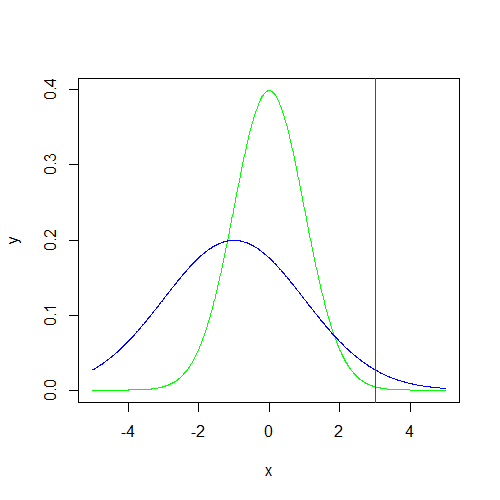
\includegraphics[width=0.5\linewidth]{normal}
\caption{Normal Means}
\end{figure}
 -
\newline \newline



\section{Support Vector Machines} 

\subsection{One-vs-One}
Since binary SVM is incentive compatible, no agent can gain from misreporting in any of the one-vs-one SVMs. Therefore, there will be no incentive to misreport in the multi-class SVM.
\newline \newline


\subsection{One-vs-Rest}
If margin is used as the prediction probabilities, then it is possible to improve the margin by misreporting the third class label, for example on the $18$-point data set.
\newline \newline


\subsection{Tree-Based}
Since binary SVM is incentive compatible, no agent can gain from misreporting in any stage. Therefore, there will be no incentive to misreport in the multi-class SVM.
\newline \newline




\section{Numerical Results} 

\subsection{Structured Examples}
A dataset is incentive incompatible with respect to the model parameterized by $w $ if at least one agent has the incentive to report $\hat{y} ^{\left(i\right)} \neq  y^{\left(i\right)}$. Formally, let the model estimated with the true label be,
\begin{align*}
w^\star  &= \arg\displaystyle\max_{w} \displaystyle\sum_{i'=1^{n}} \log\left(\mathbb{P}\left\{Y = y^{\left(i'\right)} | w, x^{\left(i'\right)}\right\}\right) + \lambda \left\|w\right\|,
\end{align*}
and the model estimated with the misreported label be,
\begin{align*}
\hat{w} &= \arg\displaystyle\max_{w} \left(\displaystyle\sum_{i' \neq  i} \log\left(\mathbb{P}\left\{Y = y^{\left(i'\right)} | w, x^{\left(i'\right)}\right\}\right)\right) + \log\left(\mathbb{P}\left\{Y = \hat{y} ^{\left(i\right)} | w, x^{\left(i\right)}\right\}\right) + \lambda \left\|w\right\|.
\end{align*}
The parameter $\lambda$ is the regulerization parameter.
\\* The dataset is incentive incompatible if there is $i $ such that,
\begin{align*}
\mathbb{P}\left\{Y = y^{\left(i\right)} | \hat{w}, x^{\left(i\right)}\right\} &> \mathbb{P}\left\{Y = y^{\left(i\right)} | w^\star , x^{\left(i\right)}\right\}.
\end{align*}
The following example with a simple structure illustrates the incentive incompatibility problem with three classes. The numerical estimation is done using the "multinom" function in R with the "nnet" library. The parameters are estimated using maximum likelihood without regularization. The estimated parameters are replicated with BFGS using the "optim" function in R with a likelihood value within $0.01$. Incentive incompatibility does not disappear when regularization with $\lambda = 0.001, 0.01$, and $0.1$ are used. The parameter estimation are done using BFGS.
\begin{figure}[H]
\centering
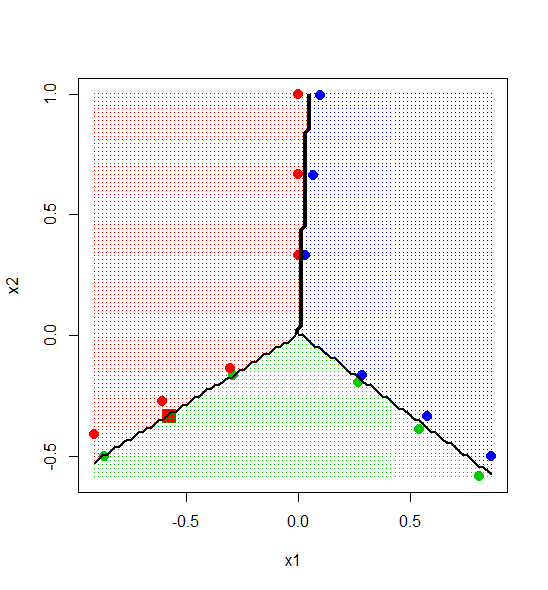
\includegraphics[width=0.5\linewidth]{test_18_8}
\caption{The 2D boundary example}
\end{figure}
 -
\\* The figure is a plot of the feature vectors of $18$ points, with their true class labels shown by colors. The classification boundary of the original model $w^\star $ with the true labels are drawn. In particular, if the agent represented by the red square report her label as blue, the probability that the point is classified as red will increase from $0.3325$ to $0.4625$.
\\* Intuitively, the agent with feature vector $x $ and label $y $ close to the classification boundary between two classes, say $y $ and $y'$, might have incentive to report the third class's label $\hat{y} \notin \left\{y , y'\right\}$ to shift the decision boundary and increase the probability that $x $ is classified as $y. $
\newline \newline
The data points are:
\begin{align*}
\left(y^{\left(1\right)}, x_{1}^{\left(1\right)}, x_{2}^{\left(1\right)}\right) &= \left(1,0.00000000,0.3333333\right)
\\ \left(y^{\left(2\right)}, x_{1}^{\left(2\right)}, x_{2}^{\left(2\right)}\right) &= \left(1,0.00000000,0.6666667\right)
\\ \left(y^{\left(3\right)}, x_{1}^{\left(3\right)}, x_{2}^{\left(3\right)}\right) &= \left(1,0.00000000,1.0000000\right)
\\ \left(y^{\left(4\right)}, x_{1}^{\left(4\right)}, x_{2}^{\left(4\right)}\right) &= \left(3,0.28867513,-0.1666667\right)
\\ \left(y^{\left(5\right)}, x_{1}^{\left(5\right)}, x_{2}^{\left(5\right)}\right) &= \left(3,0.57735027,-0.3333333\right)
\\ \left(y^{\left(6\right)}, x_{1}^{\left(6\right)}, x_{2}^{\left(6\right)}\right) &= \left(3,0.86602540,-0.5000000\right)
\\ \left(y^{\left(7\right)}, x_{1}^{\left(7\right)}, x_{2}^{\left(7\right)}\right) &= \left(2,-0.28867513,-0.1666667\right)
\\ \left(y^{\left(8\right)}, x_{1}^{\left(8\right)}, x_{2}^{\left(8\right)}\right) &= \left(1,-0.57735027,-0.3333333\right) \leftarrow \text{\;This point\;}
\\ \left(y^{\left(9\right)}, x_{1}^{\left(9\right)}, x_{2}^{\left(9\right)}\right) &= \left(2,-0.86602540,-0.5000000\right)
\\ \left(y^{\left(10\right)}, x_{1}^{\left(10\right)}, x_{2}^{\left(10\right)}\right) &= \left(3,0.03327781,0.3316681\right)
\\ \left(y^{\left(11\right)}, x_{1}^{\left(11\right)}, x_{2}^{\left(11\right)}\right) &= \left(3,0.06655561,0.6633361\right)
\\ \left(y^{\left(12\right)}, x_{1}^{\left(12\right)}, x_{2}^{\left(12\right)}\right) &= \left(3,0.09983342,0.9950042\right)
\\ \left(y^{\left(13\right)}, x_{1}^{\left(13\right)}, x_{2}^{\left(13\right)}\right) &= \left(2,0.27059406,-0.1946535\right)
\\ \left(y^{\left(14\right)}, x_{1}^{\left(14\right)}, x_{2}^{\left(14\right)}\right) &= \left(2,0.54118812,-0.3893069\right)
\\ \left(y^{\left(15\right)}, x_{1}^{\left(15\right)}, x_{2}^{\left(15\right)}\right) &= \left(2,0.81178218,-0.5839604\right)
\\ \left(y^{\left(16\right)}, x_{1}^{\left(16\right)}, x_{2}^{\left(16\right)}\right) &= \left(1,-0.30387186,-0.1370146\right)
\\ \left(y^{\left(17\right)}, x_{1}^{\left(17\right)}, x_{2}^{\left(17\right)}\right) &= \left(1,-0.60774373,-0.2740292\right)
\\ \left(y^{\left(18\right)}, x_{1}^{\left(18\right)}, x_{2}^{\left(18\right)}\right) &= \left(1,-0.91161559,-0.4110438\right)
\end{align*}
A similar example with $33$ points in which the points are away from the classification boundary. If the agent represented by the red square report her label as blue, the probability that the point is classified as red will increase from $0.8940$ to $0.8970$.
\begin{figure}[H]
\centering
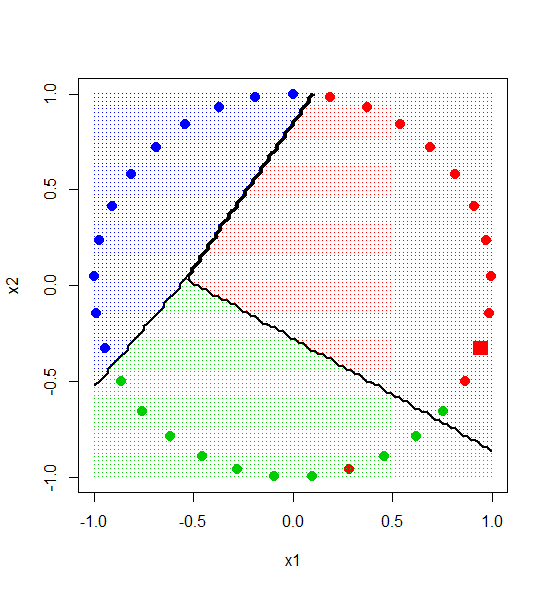
\includegraphics[width=0.5\linewidth]{test_33_15}
\caption{The 2D edge example}
\end{figure}
 -
\newline \newline
The data points are:
\begin{align*}
\left(y^{\left(1\right)}, x_{1}^{\left(1\right)}, x_{2}^{\left(1\right)}\right) &= \left(1,0.1892512,0.9819287\right)
\\ \left(y^{\left(2\right)}, x_{1}^{\left(2\right)}, x_{2}^{\left(2\right)}\right) &= \left(1,0.3716625,0.92836793\right)
\\ \left(y^{\left(3\right)}, x_{1}^{\left(3\right)}, x_{2}^{\left(3\right)}\right) &= \left(1,0.5406408,0.84125353\right)
\\ \left(y^{\left(4\right)}, x_{1}^{\left(4\right)}, x_{2}^{\left(4\right)}\right) &= \left(1,0.690079,0.72373404\right)
\\ \left(y^{\left(5\right)}, x_{1}^{\left(5\right)}, x_{2}^{\left(5\right)}\right) &= \left(1,0.814576,0.58005691\right)
\\ \left(y^{\left(6\right)}, x_{1}^{\left(6\right)}, x_{2}^{\left(6\right)}\right) &= \left(1,0.909632,0.41541501\right)
\\ \left(y^{\left(7\right)}, x_{1}^{\left(7\right)}, x_{2}^{\left(7\right)}\right) &= \left(1,0.9718116,0.23575894\right)
\\ \left(y^{\left(8\right)}, x_{1}^{\left(8\right)}, x_{2}^{\left(8\right)}\right) &= \left(1,0.9988673,0.04758192\right)
\\ \left(y^{\left(9\right)}, x_{1}^{\left(9\right)}, x_{2}^{\left(9\right)}\right) &= \left(1,0.9898214,-0.14231484\right)
\\ \left(y^{\left(10\right)}, x_{1}^{\left(10\right)}, x_{2}^{\left(10\right)}\right) &= \left(1,0.9450008,-0.32706796\right) \leftarrow \text{\;This point\;}
\\ \left(y^{\left(11\right)}, x_{1}^{\left(11\right)}, x_{2}^{\left(11\right)}\right) &= \left(1,0.8660254,-0.5\right)
\\ \left(y^{\left(12\right)}, x_{1}^{\left(12\right)}, x_{2}^{\left(12\right)}\right) &= \left(2,0.7557496,-0.65486073\right)
\\ \left(y^{\left(13\right)}, x_{1}^{\left(13\right)}, x_{2}^{\left(13\right)}\right) &= \left(2,0.618159,-0.78605309\right)
\\ \left(y^{\left(14\right)}, x_{1}^{\left(14\right)}, x_{2}^{\left(14\right)}\right) &= \left(2,0.4582265,-0.88883545\right)
\\ \left(y^{\left(15\right)}, x_{1}^{\left(15\right)}, x_{2}^{\left(15\right)}\right) &= \left(1,0.2817326,-0.95949297\right)
\\ \left(y^{\left(16\right)}, x_{1}^{\left(16\right)}, x_{2}^{\left(16\right)}\right) &= \left(2,0.09505604,-0.99547192\right)
\\ \left(y^{\left(17\right)}, x_{1}^{\left(17\right)}, x_{2}^{\left(17\right)}\right) &= \left(2,-0.09505604,-0.99547192\right)
\\ \left(y^{\left(18\right)}, x_{1}^{\left(18\right)}, x_{2}^{\left(18\right)}\right) &= \left(2,-0.2817326,-0.95949297\right)
\\ \left(y^{\left(19\right)}, x_{1}^{\left(19\right)}, x_{2}^{\left(19\right)}\right) &= \left(2,-0.4582265,-0.88883545\right)
\\ \left(y^{\left(20\right)}, x_{1}^{\left(20\right)}, x_{2}^{\left(20\right)}\right) &= \left(2,-0.618159,-0.78605309\right)
\\ \left(y^{\left(21\right)}, x_{1}^{\left(21\right)}, x_{2}^{\left(21\right)}\right) &= \left(2,-0.7557496,-0.65486073\right)
\\ \left(y^{\left(22\right)}, x_{1}^{\left(22\right)}, x_{2}^{\left(22\right)}\right) &= \left(2,-0.8660254,-0.5\right)
\\ \left(y^{\left(23\right)}, x_{1}^{\left(23\right)}, x_{2}^{\left(23\right)}\right) &= \left(3,-0.9450008,-0.32706796\right)
\\ \left(y^{\left(24\right)}, x_{1}^{\left(24\right)}, x_{2}^{\left(24\right)}\right) &= \left(3,-0.9898214,-0.14231484\right)
\\ \left(y^{\left(25\right)}, x_{1}^{\left(25\right)}, x_{2}^{\left(25\right)}\right) &= \left(3,-0.9988673,0.04758192\right)
\\ \left(y^{\left(26\right)}, x_{1}^{\left(26\right)}, x_{2}^{\left(26\right)}\right) &= \left(3,-0.9718116,0.23575894\right)
\\ \left(y^{\left(27\right)}, x_{1}^{\left(27\right)}, x_{2}^{\left(27\right)}\right) &= \left(3,-0.909632,0.41541501\right)
\\ \left(y^{\left(28\right)}, x_{1}^{\left(28\right)}, x_{2}^{\left(28\right)}\right) &= \left(3,-0.814576,0.58005691\right)
\\ \left(y^{\left(29\right)}, x_{1}^{\left(29\right)}, x_{2}^{\left(29\right)}\right) &= \left(3,-0.690079,0.72373404\right)
\\ \left(y^{\left(30\right)}, x_{1}^{\left(30\right)}, x_{2}^{\left(30\right)}\right) &= \left(3,-0.5406408,0.84125353\right)
\\ \left(y^{\left(31\right)}, x_{1}^{\left(31\right)}, x_{2}^{\left(31\right)}\right) &= \left(3,-0.3716625,0.92836793\right)
\\ \left(y^{\left(32\right)}, x_{1}^{\left(32\right)}, x_{2}^{\left(32\right)}\right) &= \left(3,-0.1892512,0.9819287\right)
\\ \left(y^{\left(33\right)}, x_{1}^{\left(33\right)}, x_{2}^{\left(33\right)}\right) &= \left(3,0,1\right)
\end{align*}
Another geometrically more symmetric example with $18$ points in which the points are away from the classification boundary. If the agent represented by the red square report her label as blue, the probability that the point is classified as red will increase from $0.3239$ to $0.4966$, which changes from an incorrect classification to the correct classification if the label with the largest prediction probability is chosen.
\begin{figure}[H]
\centering
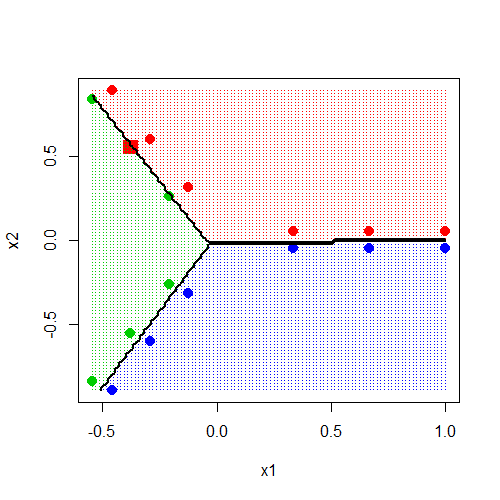
\includegraphics[width=0.5\linewidth]{test_18_5}
\caption{The 2D edge example}
\end{figure}
 -
\newline \newline
The data points are:
\begin{align*}
\left(y^{\left(1\right)}, x_{1}^{\left(1\right)}, x_{2}^{\left(1\right)}\right) &= \left(1,-0.0100000,0.3333333\right)
\\ \left(y^{\left(2\right)}, x_{1}^{\left(2\right)}, x_{2}^{\left(2\right)}\right) &= \left(1,-0.0100000,0.6666667\right)
\\ \left(y^{\left(3\right)}, x_{1}^{\left(3\right)}, x_{2}^{\left(3\right)}\right) &= \left(1,-0.0100000,1.0000000\right)
\\ \left(y^{\left(4\right)}, x_{1}^{\left(4\right)}, x_{2}^{\left(4\right)}\right) &= \left(2,-0.2836751,-0.1753269\right)
\\ \left(y^{\left(5\right)}, x_{1}^{\left(5\right)}, x_{2}^{\left(5\right)}\right) &= \left(1,-0.5723503,-0.3419936\right) \leftarrow \text{\;This point\;}
\\ \left(y^{\left(6\right)}, x_{1}^{\left(6\right)}, x_{2}^{\left(6\right)}\right) &= \left(2,-0.8610254,-0.5086603\right)
\\ \left(y^{\left(7\right)}, x_{1}^{\left(7\right)}, x_{2}^{\left(7\right)}\right) &= \left(3,0.2936751,-0.1580064\right)
\\ \left(y^{\left(8\right)}, x_{1}^{\left(8\right)}, x_{2}^{\left(8\right)}\right) &= \left(3,0.5823503,-0.3246731\right)
\\ \left(y^{\left(9\right)}, x_{1}^{\left(9\right)}, x_{2}^{\left(9\right)}\right) &= \left(3,0.8710254,-0.4913397\right)
\\ \left(y^{\left(10\right)}, x_{1}^{\left(10\right)}, x_{2}^{\left(10\right)}\right) &= \left(3,0.0100000,0.3333333\right)
\\ \left(y^{\left(11\right)}, x_{1}^{\left(11\right)}, x_{2}^{\left(11\right)}\right) &= \left(3,0.0100000,0.6666667\right)
\\ \left(y^{\left(12\right)}, x_{1}^{\left(12\right)}, x_{2}^{\left(12\right)}\right) &= \left(3,0.0100000,1.0000000\right)
\\ \left(y^{\left(13\right)}, x_{1}^{\left(13\right)}, x_{2}^{\left(13\right)}\right) &= \left(1,-0.2936751,-0.1580064\right)
\\ \left(y^{\left(14\right)}, x_{1}^{\left(14\right)}, x_{2}^{\left(14\right)}\right) &= \left(1,-0.5823503,-0.3246731\right)
\\ \left(y^{\left(15\right)}, x_{1}^{\left(15\right)}, x_{2}^{\left(15\right)}\right) &= \left(1,-0.8710254,-0.4913397\right)
\\ \left(y^{\left(16\right)}, x_{1}^{\left(16\right)}, x_{2}^{\left(16\right)}\right) &= \left(2,0.2836751,-0.1753269\right)
\\ \left(y^{\left(17\right)}, x_{1}^{\left(17\right)}, x_{2}^{\left(17\right)}\right) &= \left(2,0.5723503,-0.3419936\right)
\\ \left(y^{\left(18\right)}, x_{1}^{\left(18\right)}, x_{2}^{\left(18\right)}\right) &= \left(2,0.8610254,-0.5086603\right)
\end{align*}


\subsection{Randomly Generated Examples}
\begin{tcolorbox}[colback = white]
This section is no longer necessary.
\end{tcolorbox}
Three types of examples are randomly generated and tested for incentive incompatibility, for $m  = 1, 2$ and $k  = 2, 3, 4$
\begin{enumerate}
\item Random labels: $x_{i} \in \mathbb{R}^{m}, x_{i} \sim  N\left(0, I\right), y_{i} \sim  \text{\;Unif\;} \left[0, k - 1\right].$
\item Linearly separable labels: $x_{i} \in \mathbb{R}^{m}, x_{i} \sim  N\left(0, I\right), y_{i} = \arg\displaystyle\max_{j \in \left\{0, 1, ..., k -1\right\}} w_{j} \begin{bmatrix} x_{i} \\ 1 \end{bmatrix} , w_{j} \in \mathbb{R}^{k}, w_{j} \sim  N\left(0, I\right).$
\item Linearly separable with variance $\sigma: x_{i} \in \mathbb{R}^{m}, x_{i} \sim  N\left(0, I\right), y_{i} = \arg\displaystyle\max_{j \in \left\{0, 1, ..., k -1\right\}} w_{j} \begin{bmatrix} x_{i} \\ 1 \end{bmatrix} + \varepsilon_{j} , w_{j} \in \mathbb{R}^{k}, w_{j} \sim  N\left(0, I\right), \varepsilon \in \mathbb{R}^{k}, \varepsilon \sim  N\left(0, I\right).$
\end{enumerate}

Currently, all the following examples use the second and third methods of generating points.
\newline \newline


\subsection{One Dimensional Case}
In the case $x $ is $1$-dimensional, one randomly generated dataset with $20$ points illustrates the problem with softmax regression being not incentive compatible.
\begin{align*}
\left(x_{1}, y_{1}\right) &= \left(0.8048,2\right)
\\ \left(x_{2}, y_{2}\right) &= \left(0.5694,2\right)
\\ \left(x_{3}, y_{3}\right) &= \left(1.016,2\right)
\\ \left(x_{4}, y_{4}\right) &= \left(1.2838,2\right)
\\ \left(x_{5}, y_{5}\right) &= \left(0.0747,2\right)
\\ \left(x_{6}, y_{6}\right) &= \left(-0.4731,2\right)
\\ \left(x_{7}, y_{7}\right) &= \left(-0.5567,2\right)
\\ \left(x_{8}, y_{8}\right) &= \left(0.8745,2\right)
\\ \left(x_{9}, y_{9}\right) &= \left(-0.4735,2\right)
\\ \left(x_{10}, y_{10}\right) &= \left(-1.1037,3\right)
\\ \left(x_{11}, y_{11}\right) &= \left(1.3496,1\right)
\\ \left(x_{12}, y_{12}\right) &= \left(-0.4792,3\right)
\\ \left(x_{13}, y_{13}\right) &= \left(-0.0358,3\right)
\\ \left(x_{14}, y_{14}\right) &= \left(1.2837,1\right)
\\ \left(x_{15}, y_{15}\right) &= \left(-0.0038,2\right)
\\ \left(x_{16}, y_{16}\right) &= \left(1.4523,1\right)
\\ \left(x_{17}, y_{17}\right) &= \left(-2.3012,3\right)
\\ \left(x_{18}, y_{18}\right) &= \left(-0.3552,2\right)
\\ \left(x_{19}, y_{19}\right) &= \left(0.6926,2\right)
\\ \left(x_{20}, y_{20}\right) &= \left(0.488,2\right)
\end{align*}
If agent $4$ reports $\left(1.2838, 3\right)$, resulting in model $Y'$, instead of $\left(1.2838, 2\right)$ truthfully, resulting in model $Y, $
\begin{align*}
\mathbb{P}\left\{Y' = 2\right\} &= 0.4254 > 0.4198 = \mathbb{P}\left\{Y = 2\right\}.
\end{align*}
In the following plot, class $1, 2, 3$ has colors red, green, blue respectively. If the square green point pretends to be blue, the probability of it getting classified as green will increase.
\begin{figure}[H]
\centering
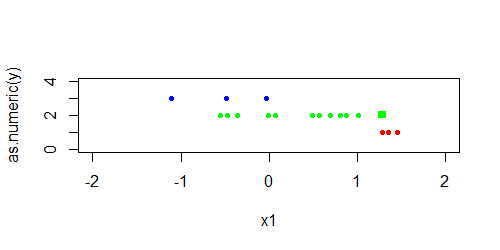
\includegraphics[width=0.5\linewidth]{test1d_421}
\caption{1D Example 1}
\end{figure}
 -
\\* A similar but linearly separable case is,
\begin{align*}
\left(x_{1}, y_{1}\right) &= \left(0.6699,3\right)
\\ \left(x_{2}, y_{2}\right) &= \left(1.3181,3\right)
\\ \left(x_{3}, y_{3}\right) &= \left(-0.724,2\right)
\\ \left(x_{4}, y_{4}\right) &= \left(0.3886,1\right)
\\ \left(x_{5}, y_{5}\right) &= \left(-1.0845,2\right)
\\ \left(x_{6}, y_{6}\right) &= \left(0.4201,3\right)
\\ \left(x_{7}, y_{7}\right) &= \left(-1.5717,2\right)
\\ \left(x_{8}, y_{8}\right) &= \left(1.8893,3\right)
\\ \left(x_{9}, y_{9}\right) &= \left(-1.3195,2\right)
\\ \left(x_{10}, y_{10}\right) &= \left(1.2162,3\right)
\\ \left(x_{11}, y_{11}\right) &= \left(-0.3737,1\right)
\\ \left(x_{12}, y_{12}\right) &= \left(-0.406,1\right)
\\ \left(x_{13}, y_{13}\right) &= \left(1.0343,3\right)
\\ \left(x_{14}, y_{14}\right) &= \left(-0.0174,1\right)
\\ \left(x_{15}, y_{15}\right) &= \left(1.4013,3\right)
\\ \left(x_{16}, y_{16}\right) &= \left(0.6972,3\right)
\\ \left(x_{17}, y_{17}\right) &= \left(1.2113,3\right)
\\ \left(x_{18}, y_{18}\right) &= \left(-1.0789,2\right)
\\ \left(x_{19}, y_{19}\right) &= \left(0.5583,3\right)
\\ \left(x_{20}, y_{20}\right) &= \left(-0.1254,1\right)
\end{align*}
If agent $4$ reports $\left(0.3886, 1\right)$, resulting in model $Y'$, instead of $\left(0.3886, 2\right)$ truthfully, resulting in model $Y, $
\begin{align*}
\mathbb{P}\left\{Y' = 2\right\} &= 0.7736 > 0.6353 = \mathbb{P}\left\{Y = 2\right\}.
\end{align*}
In the following plot, class $1, 2, 3$ has colors red, green, blue respectively. If the square red point pretends to be green, the probability of it getting classified as red will increase.
\begin{figure}[H]
\centering
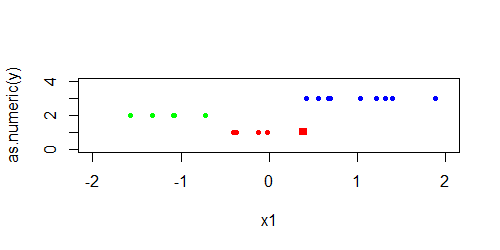
\includegraphics[width=0.5\linewidth]{test1d_585}
\caption{1D Example 2}
\end{figure}
 -
\newline \newline


\subsection{Two Dimensional Case}
One example in which the data is not linearly separable:
\begin{align*}
\left(x_{1,1}, x_{2,1}, y\right) &= \left(-0.2078, 1.7184, 1\right)
\\ \left(x_{1,2}, x_{2,2}, y\right) &= \left(-0.648, -0.1972, 1\right)
\\ \left(x_{1,3}, x_{2,3}, y\right) &= \left(-1.551, 0.2337, 1\right)
\\ \left(x_{1,4}, x_{2,4}, y\right) &= \left(0.5005, 0.0292, 2\right)
\\ \left(x_{1,5}, x_{2,5}, y\right) &= \left(0.6556, 0.2169, 2\right)
\\ \left(x_{1,6}, x_{2,6}, y\right) &= \left(-0.7498, -0.0237, 1\right)
\\ \left(x_{1,7}, x_{2,7}, y\right) &= \left(0.3018, 0.2766, 2\right)
\\ \left(x_{1,8}, x_{2,8}, y\right) &= \left(-0.6075, 1.8255, 1\right)
\\ \left(x_{1,9}, x_{2,9}, y\right) &= \left(0.093, 0.0902, 3\right)
\\ \left(x_{1,10}, x_{2,10}, y\right) &= \left(-0.341, 0.3715, 2\right)
\\ \left(x_{1,11}, x_{2,11}, y\right) &= \left(-0.1007, 0.4598, 2\right)
\\ \left(x_{1,12}, x_{2,12}, y\right) &= \left(0.6475, 1.8673, 2\right)
\\ \left(x_{1,13}, x_{2,13}, y\right) &= \left(0.0962, 1.5949, 2\right)
\\ \left(x_{1,14}, x_{2,14}, y\right) &= \left(-1.1301, 0.9306, 1\right)
\\ \left(x_{1,15}, x_{2,15}, y\right) &= \left(-1.6144, 0.5291, 1\right)
\\ \left(x_{1,16}, x_{2,16}, y\right) &= \left(1.3819, 0.5892, 2\right)
\\ \left(x_{1,17}, x_{2,17}, y\right) &= \left(0.3037, -1.255, 3\right)
\\ \left(x_{1,18}, x_{2,18}, y\right) &= \left(-0.275, -1.1986, 3\right)
\\ \left(x_{1,19}, x_{2,19}, y\right) &= \left(0.9622, -0.103, 3\right)
\\ \left(x_{1,20}, x_{2,20}, y\right) &= \left(-0.2279, -0.5819, 3\right)
\end{align*}
If agent $4$ reports $\left(0.5005, 0.0292, 1\right)$, resulting in model $Y'$, instead of $\left(0.5005, 0.0292, 2\right)$ truthfully, resulting in model $Y, $
\begin{align*}
\mathbb{P}\left\{Y' = 2\right\} &= 0.4681 > 0.4548 = \mathbb{P}\left\{Y = 2\right\}.
\end{align*}
In the following plot, class $1, 2, 3$ has colors red, green, blue respectively. If the square red point pretends to be a green point, the probability of it getting classified as red will increase.
\begin{figure}[H]
\centering
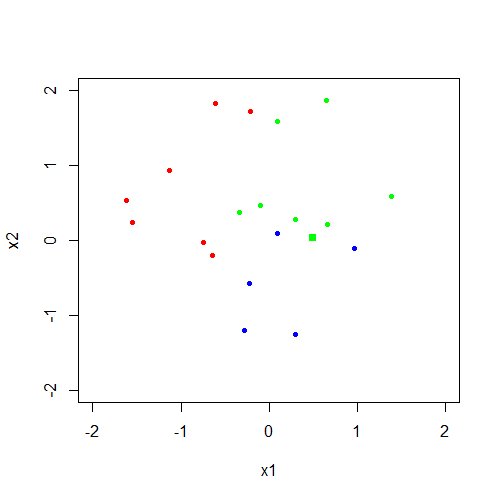
\includegraphics[width=0.5\linewidth]{test2d_217}
\caption{2D Example 1}
\end{figure}
 -
\newline \newline
One example in which the data is linearly separable:
\begin{align*}
\left(x_{1,1}, x_{2,1}, y\right) &= \left(0.0684, 1.2528, 1\right)
\\ \left(x_{1,2}, x_{2,2}, y\right) &= \left(-0.8979, 1.7309, 1\right)
\\ \left(x_{1,3}, x_{2,3}, y\right) &= \left(-0.0656, -1.6169, 2\right)
\\ \left(x_{1,4}, x_{2,4}, y\right) &= \left(1.1107, -0.6537, 3\right)
\\ \left(x_{1,5}, x_{2,5}, y\right) &= \left(0.2553, 1.4098, 1\right)
\\ \left(x_{1,6}, x_{2,6}, y\right) &= \left(1.3888, 0.8675, 2\right)
\\ \left(x_{1,7}, x_{2,7}, y\right) &= \left(0.4308, -0.8872, 2\right)
\\ \left(x_{1,8}, x_{2,8}, y\right) &= \left(1.5898, 1.468, 2\right)
\\ \left(x_{1,9}, x_{2,9}, y\right) &= \left(0.6773, 2.2383, 1\right)
\\ \left(x_{1,10}, x_{2,10}, y\right) &= \left(-0.5839, -0.071, 1\right)
\\ \left(x_{1,11}, x_{2,11}, y\right) &= \left(0.2665, 0.4818, 2\right)
\\ \left(x_{1,12}, x_{2,12}, y\right) &= \left(-0.8833, -0.6374, 1\right)
\\ \left(x_{1,13}, x_{2,13}, y\right) &= \left(0.0716, -1.082, 2\right)
\\ \left(x_{1,14}, x_{2,14}, y\right) &= \left(-0.512, -0.1667, 1\right)
\\ \left(x_{1,15}, x_{2,15}, y\right) &= \left(1.353, -0.0793, 3\right)
\\ \left(x_{1,16}, x_{2,16}, y\right) &= \left(-0.6957, -0.1058, 1\right)
\\ \left(x_{1,17}, x_{2,17}, y\right) &= \left(0.2837, -0.8186, 2\right)
\\ \left(x_{1,18}, x_{2,18}, y\right) &= \left(0.8643, -1.1354, 2\right)
\\ \left(x_{1,19}, x_{2,19}, y\right) &= \left(1.2658, 0.9953, 2\right)
\\ \left(x_{1,20}, x_{2,20}, y\right) &= \left(-1.6236, 0.0485, 1\right)
\end{align*}
If agent $18$ reports $\left(0.8643, -1.1354, 1\right)$, resulting in model $Y'$, instead of $\left(0.8643, -1.1354, 2\right)$ truthfully, resulting in model $Y, $
\begin{align*}
\mathbb{P}\left\{Y' = 2\right\} &= 0.9213 > 0.9098 = \mathbb{P}\left\{Y = 2\right\}.
\end{align*}
In the following plot, class $1, 2, 3$ has colors red, green, blue respectively. If the square red point pretends to be a green point, the probability of it getting classified as red will increase.
\begin{figure}[H]
\centering
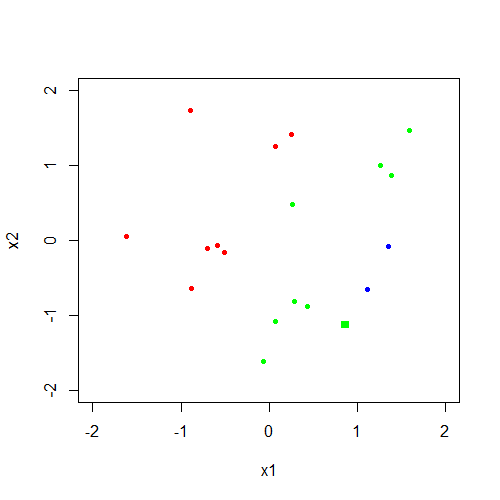
\includegraphics[width=0.5\linewidth]{test2d_1805}
\caption{2D Example 2}
\end{figure}
 -
\newline \newline
\bibliographystyle{te}
\bibliography{cs}


\end{document}
